\documentclass[aps,prd,preprint,floats,epsf,superscriptaddress,nofootinbib]{revtex4}
%\documentclass[aps,prd,twocolumn,superscriptaddress,preprintnumbers]{revtex4}


\usepackage{amsmath,amssymb,amsthm,amsfonts} % general AMS maths resource packages
\usepackage{bm} % bold math
\usepackage{bbm} % bold math for {\mathbbm 1}
\usepackage{braket} % Dirac bracket notation for quantum physics
\usepackage{cancel} % cancel terms to something
%\usepackage{caption} % use subfigure environments inside a figure environment
%\usepackage{subcaption} % use subfigure environments inside a figure environment
\usepackage{color}
\usepackage{dcolumn} % align table columns on decimal point
\usepackage{dsfont}
\usepackage{empheq} % boxed equation
\usepackage{enumitem} % enumerate items in different ways
%\usepackage{epsfig,showkeys}
\usepackage{graphicx} % packages to allow inclusion of graphics
\usepackage{indentfirst}
\usepackage[utf8]{inputenc} % useful to type directly diacritic characters
\usepackage{marginnote}
\usepackage{mathrsfs}
\usepackage{mathtools} % in order to use \Aboxed
\usepackage{multirow}
\usepackage{setspace} % set line spacing
\usepackage{simpler-wick} % Wick contraction
\usepackage{slashed} % Feynman slashes
%\usepackage[skins,breakable]{tcolorbox} % breakable box
\usepackage{subfigure} % use subfigures
\usepackage[most]{tcolorbox} % breakable box
\usepackage{tikz} % draw commutative diagrams
\usetikzlibrary{matrix}
\usepackage{ulem}
\usepackage{wrapfig} % wrap text around figures
\usepackage{xcolor}
\usepackage[vcentermath]{youngtab} % draw Young tableaux
\usepackage{ytableau} % draw Young tableaux, better than youngtab



\usepackage[T1]{fontenc}
\usepackage{calligra}
\usepackage[T1]{pbsi}
\usepackage{CJKutf8} % Chinese typing


%\usepackage[left=1cm,top=1cm,bottom=1cm,right=1cm,nohead,nofoot]{geometry} % margins
\usepackage[colorlinks,
            linkcolor=black,
            anchorcolor=black,
            citecolor=black,
%            linktoc=all
            ]{hyperref} % For creating hyperlinks in cross references
%\usepackage[linktoc=all]{hyperref}
\definecolor{wine-stain}{rgb}{0.5,0,0}
\hypersetup{
  colorlinks,
  linkcolor=blue,
%  linkcolor=wine-stain,
  linktoc=all
}


\newtheorem{theorem}{Theorem}[section]
\newtheorem{corollary}{Corollary}[theorem]
\newtheorem{lemma}[theorem]{Lemma}


\newcommand{\eg}{{\it e.g.}}
\newcommand{\ie}{{\it i.e.}}
\newcommand{\cf}{{\it cf}}
\newcommand{\re}{{\rm Re}}
\newcommand{\im}{{\rm Im}}
\newcommand{\parallelsum}{\mathbin{\!/\mkern-5mu/\!}}
\newcommand{\blue}[1]{\color{blue} #1}
\newcommand{\red}[1]{\color{red} #1}
\newcommand{\tr}{\operatorname{tr}}






%%%%%%%%%%%%%%%%%%%%%%%%%%%%%%%%%%%%%%%%%%%%%%%%%%%%%%%%%%%%
%\topmargin 0in
%\textheight 8.7in
%\textwidth 6.2in
%\hoffset -0.4in

\begin{document}

\bigskip
\title{\bf Quantum Teleportation: \\ Protocol, Implementation, and Applications}
\bigskip

\author{Ying-Han Su, Ting-Peng Huang, Po-Rui Chen}
\email[e-mail: ]{b11303052@ntu.edu.tw}
\affiliation{Department of Physics, National Taiwan University, Taipei, Taiwan 10617, R.O.C.}

\date{\today}

\begin{abstract}
This report provides a comprehensive study of quantum teleportation, covering its protocol, implementation, and applications. We begin with an introduction to the fundamental concepts and historical development of quantum teleportation. We then present the theoretical framework and the step-by-step protocol for achieving quantum teleportation. Following this, we discuss various implementation strategies and their practical challenges. Finally, we explore the current and potential applications of quantum teleportation in quantum information processing and communication.
\end{abstract}

\maketitle

\tableofcontents


%%%%%%%%%%%%%%%%%%%%%%%%%%%%%%%%%%%%%%%%%%%%%%%%%%
\newpage

\section{Introduction}
\label{sec:introduction}
%%%%%%%%%%%%%%%%%%%%%%%%%%%%%%%%%%%%%%%%%%%%%%%%%%

%%%%%%%%%%%%%%%%%%%%%%%%%%%%%%%%%%%%%%%%%%%%%%%%%%
\newpage
\section{Mathematical background}
\label{sec:math background}
%%%%%%%%%%%%%%%%%%%%%%%%%%%%%%%%%%%%%%%%%%%%%%%%%%
\subsection{Qubits and the Hilbert Space Formalism}
The fundamental unit of quantum information is the "qubit". Unlike classical bit, which takes the value of either 0 or 1 at one of the time, a qubit exists in a two-dimensional Hilbert space $\mathcal{H}=\mathrm{span}\{|0\rangle, |1\rangle\} \cong \mathbb{C}^2$, and its state can be described by a unit vector with an orthonormal computational basis $\{|0\rangle, |1\rangle\}$ \begin{equation}
  |\psi\rangle = \alpha|0\rangle+\beta|1\rangle, \ \alpha, \beta \in \mathbb{C}, \  |\alpha|^2+|\beta|^2=1
  \label{Eq: qubit}
\end{equation}
where $\alpha$ and $\beta$ are the probability amplitudes: measurement yielding $|0\rangle$ or $|1\rangle$ has a probability $|\alpha|^2$ and $|\beta|^2$, respectively  ~\cite{NielsenChuang2000}. Unlike classical bit, a qubit can exist in a superposition of both states, which has no classical analogue. Physical realization of qubits include the two polarization of photon and two energy levels of an electron in an atom. 

\textbf{Bloch Sphere} As an phase factor $e^{i\gamma}$ does not have observable effect, Eq.~\ref{Eq: qubit} can be written in a more general expression \begin{equation}
  \ket{\psi} = \cos{\frac{\theta}{2}}\ket{0}+e^{i \varphi}\sin{\frac{\theta}{2}}\ket{1}, \ \theta\in[0,\pi], \ \varphi \in[0,2\pi) 
\end{equation} 
The two parameters $\theta$ and $\varphi$ define a unique point on the unit three-dimensional sphere, known as the Bloch sphere as shown in Figure~\ref{fig:bloch sphere}.
\begin{figure}[h]
    \centering
    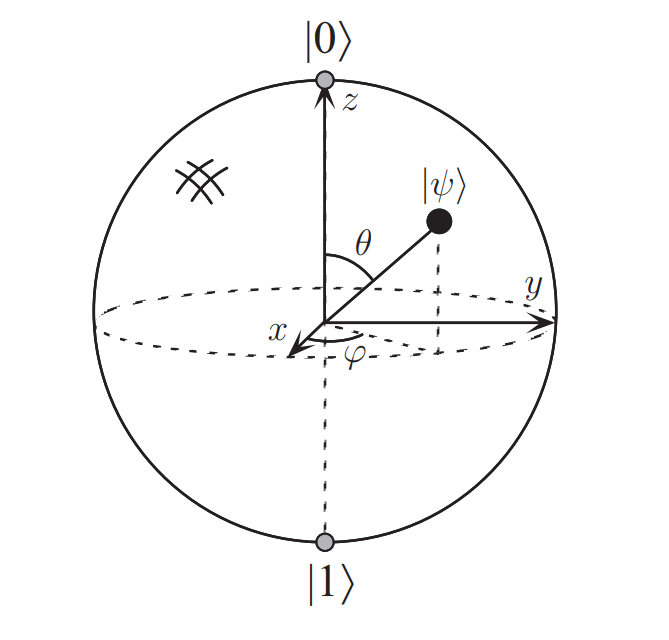
\includegraphics[width=0.5\textwidth]{figures/bloch sphere.png}
    \caption{Bloch sphere schematic. An arbitrary qubit can be represented by one point on the sphere~\cite{NielsenChuang2000}.}
    \label{fig:bloch sphere}
\end{figure} 
The north pole ($\theta=0$) corresponds to $\ket{0}$, while the south polt corresponds to $\ket{1}$, and every point on the equator represents an equal superposition such as $\ket{+}=(\ket{0}+\ket{1})/\sqrt{2}$. 

\textbf{Multi-qubit systems}. For a system of two qubits, we use the tensor product of the individual Hilbert space $\mathcal{H}_{12}=\mathcal{H}_1\otimes\mathcal{H}_2 \cong \mathbb{C}^4$ to represent the state space, with computational basis kets $\{\ket{00},\ket{01},\ket{10},\ket{11}\}$. Here we use the ordering convention. That is, $\ket{01}=\ket{0}_1\otimes\ket{1}_1$. Similarly, if it is a system of three qubits, then $\ket{010}=\ket{0}_1\otimes\ket{1}_2\otimes\ket{0}_2$. A general two-qubit state takes the form \begin{equation}
  \ket{\psi}=\alpha_{00}\ket{00}+\alpha_{01}\ket{01}+\alpha_{10}\ket{10}+\alpha_{11}\ket{11}, \ \sum_x|\alpha_x|^2=1
\end{equation}

\subsection{Entanglement and the Bell States}
A two-qubit state is called separable if it can be factored as $\ket{\psi \phi}=\ket{\psi}_A\otimes\ket{\psi}_B$. This means that qubit A is in state $\ket{\psi}$, while qubit B is in state $\ket{\phi}$. On the other hand, an entangled state can not be factorized into the product of two single-qubit states. In this case, the quantum state can only be understood as a property of the whole system. 
The most important entangled states for quantum teleportation are the Bell states~\cite{NielsenChuang2000, Bennett}\begin{equation}
\begin{aligned}
|\Phi^+\rangle &= \frac{1}{\sqrt{2}}(|00\rangle + |11\rangle), 
&\quad |\Phi^-\rangle &= \frac{1}{\sqrt{2}}(|00\rangle - |11\rangle) \\[6pt]
|\Psi^+\rangle &= \frac{1}{\sqrt{2}}(|01\rangle + |10\rangle), 
&\quad |\Psi^-\rangle &= \frac{1}{\sqrt{2}}(|01\rangle - |10\rangle).
\end{aligned}
\end{equation}
These four states form an orthonormal basis for the two-qubit Hilbert space. Besides, they are maximally entangled: tracing out either qubit leaves the reduced density matrix $\rho=I/2$, where $I$ is the identity matrix. For example, consider the Bell state $\ket{\Phi^+}_{AB}$, then the corresponding density matrix is $\rho_{AB}=\ket{\Phi^+}\bra{\Phi^+}$. Now, if we only look at the qubit A subsystem, we trace out qubit B to get the reduced density matrix as \begin{equation}
  \rho_A=\tr_B(\rho_{AB})=\frac{I_A}{2}.
\end{equation} Similarly, we have $\rho_B=\frac{I_B}{2}$. This implies that when measuring either qubit, we get equal probability of getting $\ket{0}$ or $\ket{1}$. However, the measurement results of system A and system B are perfectly correlated. For example, if system A measure the entangled state and gets $\ket{0}$, then B gets $\ket{0}$. Similarly, if A obtains $\ket{1}$, then B gets $\ket{1}$. That is, each local measurement result is random, but it becomes highly correlated once we look at the system as a whole.
\subsection{Quantum Measurement and Bell Measurement} The projection postulate state that measurement irreversibly collapses the superposition state into one of its components~\cite{Bouwmeester}. Therefore, measurement on the qubit is a physical process that will disturb the original state. A projective measurement is described by a Hermitian observable $M=\sum_m mP_m$, where $\{P_m\}$ are orthogonal projection operator onto the eigenspace of $M$ with eigenvalue $m$ and satisfy $\sum_m P_m=I$ and $P_mP_{m'}=\delta_{mm'}P_m$. Given a pure state $\ket{\psi}$, the probability of obtaining outcome $m$ is \begin{equation}
  p(m)=\bra{\psi}P_m\ket{\psi}
\end{equation}
and the post-measurement state collapses to~\cite{NielsenChuang2000} \begin{equation}
  \ket{\psi_m}=\frac{P_m\ket{\psi}}{\sqrt{p(m)}}.
  \label{Eq:post-measurement normalization}
\end{equation} For example, consider a qubit $\ket{\psi}=\alpha\ket{0}+\beta\ket{1}$ with $|\alpha|^2+|\beta|^2=1$. If we do the measurement in the computational basis $\{\ket{0},\ket{1}\}$, then the corresponding projection operators are $P_0=\ket{0}\bra{0}, \ P_1=\ket{1}\bra{1}$. The probability and the post-measurement states of the two possible outcomes are \begin{equation}
  \begin{aligned}
    p(0)&=\bra{\psi}P_0\ket{\psi}=|\alpha|^2, 
&\quad P_0\ket{\psi}&=\ket{0}\bra{0}(\alpha\ket{0}+\beta\ket{1})=\alpha\ket{0}\\
p(1)&=\bra{\psi}P_1\ket{\psi}=|\beta|^2,
&\quad  P_1\ket{\psi}&=\ket{1}\bra{1}(\alpha\ket{0}+\beta\ket{1})=\beta\ket{1}.\\
  \end{aligned}
\end{equation} Therefore, a direct measurement gives either 0 or 1, and the original coefficients disappear due to the normalization (Equation~\ref{Eq:post-measurement normalization}), and thus the original qubit state is no longer available.
In order to maintain the original qubit state, in quantum teleportation, a Bell measurement is performed on a two-qubit system. Similar to the projective measurement, we define the Bell-measurement projectors as \begin{equation}
  P_k=\ket{\beta_k}\bra{\beta_k}, \ \ket{\beta_k}\in\{\ket{\Psi^{\pm}},\ket{\Phi^{\pm}}\}.
\end{equation} Thus, a Bell measurement yields one of the Bell states. That is, computational-basis measurement tells us whether each qubit is individually in $\ket{0}$ or $\ket{1}$, while a Bell measurement implies which Bell state the two-qubit system occupies as a whole. 
\subsection{Pauli Operators and Unitary Correction}
The Pauli operators are a set of $2\times2$ unitary matrices forming a basis for the space of single-qubit operators~\cite{NielsenChuang2000}:\begin{equation}
\begin{aligned}
I = \left(\begin{array}{cc} 1 & 0 \\ 0 & 1 \end{array}\right),
&\qquad X = \sigma_1=\left(\begin{array}{cc} 0 & 1 \\ 1 & 0 \end{array}\right), \\[10pt]
Z = \sigma_3=\left(\begin{array}{cc} 1 & 0 \\ 0 & -1 \end{array}\right),
&\qquad Y =\sigma_2= iXZ = \left(\begin{array}{cc} 0 & -i \\ i & 0 \end{array}\right).
\end{aligned}
\end{equation}These are the standard single-qubit Pauli operators used in the quantum information. In particular, $X$ is a bit-flip operator ($X\ket{0}=\ket{1},\ X\ket{1}=\ket{0}$), $Z$ acts as a phase-flip operator ($Z\ket{0}=\ket{0}, \ Z\ket{1}=-\ket{1}$), while $Y$ is the same operator as $XZ$ up to a phase factor. Therefore, we will just use $XZ$ in the later protocal operation. These four operators $\{I,\ X,\ Z,\ XZ\}$ will serve as the unitary correction operators for Bob to recover the original quantum state after Alice's Bell measurement.
%%%%%%%%%%%%%%%%%%%%%%%%%%%%%%%%%%%%%%%%%%%%%%%%%%
\newpage
\section{Standard quauntum teleportation protocal}
\label{sec:protocal}
In this chapter, we use the mathmatical tools introduced in the previous chapter to derive the standard quantum teleportation protocal. The goal of the protocol is to transfer an unknown quantum state from Alice to Bob without physically sending the original qubit through a quantum channel. Instead, the protocol uses one shared Bell pair, one Bell measurement, two bits of classical communication, and a conditional Pauli correction.

Suppose Alice has an unknown qubit state \begin{equation}
  \ket{\psi}_1=\alpha\ket{0}_1+\beta\ket{1}_1,\ |\alpha|^2+|\beta|^2=1.
\end{equation} Here the subscript 1 labels the unknown input qubit. Alice does not know the coefficients, and she may not measure it directly as the post-measurement state would collapse. Therefore, Alice and Bob share an entangled Bell pair, say \begin{equation}
  \ket{\Phi^+}_{23}=\frac{1}{\sqrt{2}}(\ket{00}_{23}+\ket{11}_{23}),
\end{equation} where qubit 2 and 3 are held by Alice and Bob respectively. The total initial state of the three-qubit system is \begin{equation}
  \begin{aligned}
    \ket{\Psi}_{123}&=\ket{\psi}_1\ket{\Phi^+}_{23}\\
    &=\frac{1}{\sqrt{2}}\left(\alpha\ket{000}_{123}+\alpha\ket{011}_{123}+\beta\ket{100}_{123}+\beta\ket{111}_{123}\right),
  \end{aligned}
\end{equation}where in the second line of the equation we expand the total qubit state. Since Alice will perform a Bell measurement on qubit 1 and 2, this suggests us to express the computational basis $\ket{}_{12}$ in terms of the Bell states as \begin{equation}
\begin{aligned}
\ket{00}_{12}
&=
\frac{1}{\sqrt{2}}
\left(
\ket{\Phi^+}_{12}
+
\ket{\Phi^-}_{12}
\right),
&\qquad
\ket{11}_{12}
&=
\frac{1}{\sqrt{2}}
\left(
\ket{\Phi^+}_{12}
-
\ket{\Phi^-}_{12}
\right),
\\[10pt]
\ket{01}_{12}
&=
\frac{1}{\sqrt{2}}
\left(
\ket{\Psi^+}_{12}
+
\ket{\Psi^-}_{12}
\right),
&\qquad
\ket{10}_{12}
&=
\frac{1}{\sqrt{2}}
\left(
\ket{\Psi^+}_{12}
-
\ket{\Psi^-}_{12}
\right).
\end{aligned}
\label{Eq:computational_to_Bell}
\end{equation} Thus, the total state becomes \begin{equation}
\begin{aligned}
\ket{\psi}_1\ket{\Phi^+}_{23}
=
\frac{1}{2}
\bigg[
&\ket{\Phi^+}_{12}
\left(
\alpha\ket{0}_3
+
\beta\ket{1}_3
\right)
+
\ket{\Phi^-}_{12}
\left(
\alpha\ket{0}_3
-
\beta\ket{1}_3
\right)
\\
&+
\ket{\Psi^+}_{12}
\left(
\beta\ket{0}_3
+
\alpha\ket{1}_3
\right)
+
\ket{\Psi^-}_{12}
\left(
-\beta\ket{0}_3
+
\alpha\ket{1}_3
\right)
\bigg].
\end{aligned}
\label{Eq:teleportation_expanded_Bell_basis}
\end{equation} We may further rewrite this expression using the Pauli operators as \begin{equation}
\ket{\psi}_1\ket{\Phi^+}_{23}
=
\frac{1}{2}
\left[
\ket{\Phi^+}_{12}\ket{\psi}_3
+
\ket{\Phi^-}_{12}Z\ket{\psi}_3
+
\ket{\Psi^+}_{12}X\ket{\psi}_3
+
\ket{\Psi^-}_{12}XZ\ket{\psi}_3
\right].
\label{Eq:teleportation_identity}
\end{equation}
This equation is the central identity of quantum teleportation. It shows that when qubits 1 and 2 are written in the Bell basis, Bob's qubit 3 is related to the original input state by one of four possible Pauli operations. Alice now perform a Bell measurement on qubits 1 and 2. According to the projection postulate, the total state collapses into one of the four Bell states with equal probability. If Alice obtains the outcome $\ket{\Phi^+}_{12}$, then Bob's qubit is simply $\ket{\psi}_3$. With no extra correction, the unknown qubit is teleported to Bob. If Alice get $\ket{\Phi^-}_{12}$, then Bob's qubit is $Z\ket{\psi}_3$. Bob need to apply $Z$ so that $Z(Z\ket{\psi}_3)=Z^2\ket{\psi}_3=\ket{\psi}_3$. Similarly, if Alice obtains $\ket{\Psi^+}_{12}$, Bob gets $X\ket{\psi}_3$ and need to perform $X$ so that $X(X\ket{\psi}_3)=X^2\ket{\psi}_3=\ket{\psi}_3$. Finally, if Alice obtains $\ket{\Psi^-}_{12}$, Bob apply $ZX$ such that $ZX(XZ\ket{\psi}_3)=\ket{\psi}_3$. These four cases can be summarized into the following table as \begin{equation}
\begin{array}{c|c|c}
\text{Alice's Bell outcome} 
& \text{Bob's state before correction} 
& \text{Bob's correction} \\
\hline
\ket{\Phi^+}_{12} & \ket{\psi}_3 & I \\
\ket{\Phi^-}_{12} & Z\ket{\psi}_3 & Z \\
\ket{\Psi^+}_{12} & X\ket{\psi}_3 & X \\
\ket{\Psi^-}_{12} & XZ\ket{\psi}_3 & ZX
\end{array}
\label{Eq:teleportation_correction_table}
\end{equation}
After Alice's measurement, she need to tell Bob which one of these four Bell states she got. Since one classical bit has two possible values, 0 and 1, two classical bits can represent four possible messages: 00, 01, 10, and 11. This is enough to label the four Bell-measurement outcomes. For example, they may agree that 00 correspons to $\ket{\Phi^+}_{12}$. That is, with a two-classical-bit channel, Alice can transport her measurement result to Bob so that he can perform the corresponding correction operation to get the original unknown qubit state. In source language, the teleportation protocal can be summarized as
\begin{equation}
  1\ \mathrm{ebit}+2\ \mathrm{classical \ bits}\to 1 \mathrm{transmitted\ qubit}.
\end{equation}
%%%%%%%%%%%%%%%%%%%%%%%%%%%%%%%%%%%%%%%%%%%%%%%%%%

%%%%%%%%%%%%%%%%%%%%%%%%%%%%%%%%%%%%%%%%%%%%%%%%%%
\newpage
\section{Physical meaning and experimental relevance}
\label{sec:Physical meaning}
After deriving the standard teleportation protocol, it is important to clarify what the protocol does and does not imply physically. Quantum teleportation transfers an unknown quantum state from Alice's qubit to Bob's qubit, but it does not transfer matter, does not create a second copy of the state, and does not allow faster-than-light communication. The protocol works only because of the shared entangled pair and a classical bit channel. In this section, we discuss these physical implications and then connect the ideal protocol to experimental realization.
\subsection{No-Cloning}
Quantum teleportation does not create a second copy of the unknown quantum state. Although Bob's final qubit becomes $\ket{\psi}_3 = \alpha\ket{0}_3 + \beta\ket{1}_3$, Alice's original qubit is no longer available after the Bell measurement. The Bell measurement projects qubits 1 and 2 into one of the four Bell 
states, and therefore irreversibly destroys the original unknown state 
on Alice's side. This is why quantum teleportation is consistent with the no-cloning 
theorem. The no-cloning theorem, first formulated by Wootters and 
Zurek~\cite{Wootters1982} and independently by Dieks~\cite{Dieks1982}, 
states that it is impossible to make an exact copy of an arbitrary 
unknown quantum state. The proof is straightforward. Suppose there 
exists a universal unitary cloning machine $U$ such that
$U\ket{\psi}\ket{s} = \ket{\psi}\ket{\psi}$ for any unknown state $\ket{\psi}$, where $\ket{s}$ is a blank initial 
state. If the same machine can also clone another state $\ket{\phi}$, 
then $U\ket{\phi}\ket{s} = \ket{\phi}\ket{\phi}.$
Taking the inner product of these two equations gives
$\braket{\psi|\phi} = \braket{\psi|\phi}^{2}.$
This condition is only satisfied when $\braket{\psi|\phi}=0$ or 
$\braket{\psi|\phi}=1$. In other words, the two states must be either 
orthogonal or identical. Therefore, no single unitary operation can 
clone an arbitrary unknown quantum state~\cite{NielsenChuang2000}.

Teleportation avoids this contradiction because it does not copy the 
state. Instead, the quantum information initially contained in qubit 1 
is transferred to qubit 3, while the original state at Alice's side is 
destroyed by measurement. Therefore, teleportation should be understood 
as state transfer rather than state duplication.
\subsection{No Faster-Than-Light Communication}
Quantum teleportation also does not allow faster-than-light 
communication. Although the shared Bell pair provides nonclassical correlations between Alice and Bob, Bob cannot recover the unknown state before receiving Alice's classical message. That is, Bob needs Alice's message so that he knows what operation he should apply to recover the unkown qubit. 
This can be made more precise by looking at Bob's reduced density matrix 
before the classical message arrives. Since the four Bell-measurement 
outcomes occur with equal probability, Bob's local state is an average 
over the four possible states:
\begin{equation}
    \rho_3 = \frac{1}{4}\left(
    \ket{\psi}\bra{\psi}
    + Z\ket{\psi}\bra{\psi}Z
    + X\ket{\psi}\bra{\psi}X
    + XZ\ket{\psi}\bra{\psi}ZX
    \right).
\end{equation}
For an arbitrary qubit $\ket{\psi}=\alpha\ket{0}+\beta\ket{1}$, 
this average becomes
\begin{equation}
    \rho_3 = \frac{I}{2}.
\end{equation}
Thus, before receiving Alice's classical message, Bob's local state is 
completely mixed and independent of $\alpha$ and $\beta$. Any 
measurement Bob performs locally gives random results and reveals no information about the unknown input state. Bennett et al.~\cite{Bennett} emphasized this point in the original teleportation paper: if Bob tries to complete the protocol by guessing Alice's classical message before it arrives, his state is only a maximally mixed state and gives no information about the input state.
\subsection{Security of the Classical Message}
%%%%%%%%%%%%%%%%%%%%%%%%%%%%%%%%%%%%%%%%%%%%%%%%%%
\newpage
\section{Experimental Implementation via Dual-Photon Entanglement}

\subsection{The Quantum Leap from Theory to Lab}
The 1998 experiment by Boschi et al. marked a paradigm shift in realizing quantum information protocols. While the canonical Bennett et al. (1993) model required three independent photons—posing formidable temporal synchronization hurdles—this design utilized a sophisticated two-photon, dual-degree-of-freedom architecture. By exploiting both the momentum (path or k-vector) and polarization of a single entangled photon pair, researchers accessed a four-dimensional Hilbert space ($2 \text{ paths} \times 2 \text{ polarizations}$) within a bipartite system. This architectural innovation addressed two primary limitations of prior configurations:

\begin{itemize}
    \item \textbf{100\% Success Rate in Bell State Measurement:} Unlike linear-optics three-photon schemes (bounded by a 50\% success rate), this approach permits projection onto the complete Bell basis, enabling the deterministic identification of all four states simultaneously.
    \item \textbf{Elimination of Three-Photon Coincidence Hurdles:} Deriving the entire process from a single entangled photon pair (EPR source) circumvents the prohibitive difficulty of synchronizing independent sources within sub-nanosecond coincidence windows.
\end{itemize}

The physical execution initiates at the EPR source, where the non-local quantum channel is established.

\subsection{Implementation of the Dual-Degree-of-Freedom Setup}

\subsubsection{The EPR Source: Converting Light into Entanglement}
Entanglement is generated via Type-II spontaneous parametric down-conversion (SPDC). Specifically, a 200 mW, 351.1 nm ultraviolet argon laser pumps a $\beta$-barium borate (BBO) crystal, producing polarization-entangled photon pairs at 702.2 nm. To facilitate the dual-degree architecture, this initial polarization entanglement is deterministically converted into spatial path entanglement via birefringent calcite crystals (C), which split the incident photons into discrete spatial paths ($a$ and $b$). The resulting EPR state is described by:
$$|\Psi\rangle=\frac{1}{\sqrt{2}}(|a_1\rangle|a_2\rangle+|b_1\rangle|b_2\rangle)$$

Crucially, photon 1 is routed toward Alice's station, while photon 2 traverses backreflected paths $a_2$ and $b_2$ through the BBO crystal toward Bob.


\begin{figure}[h]
    \centering
    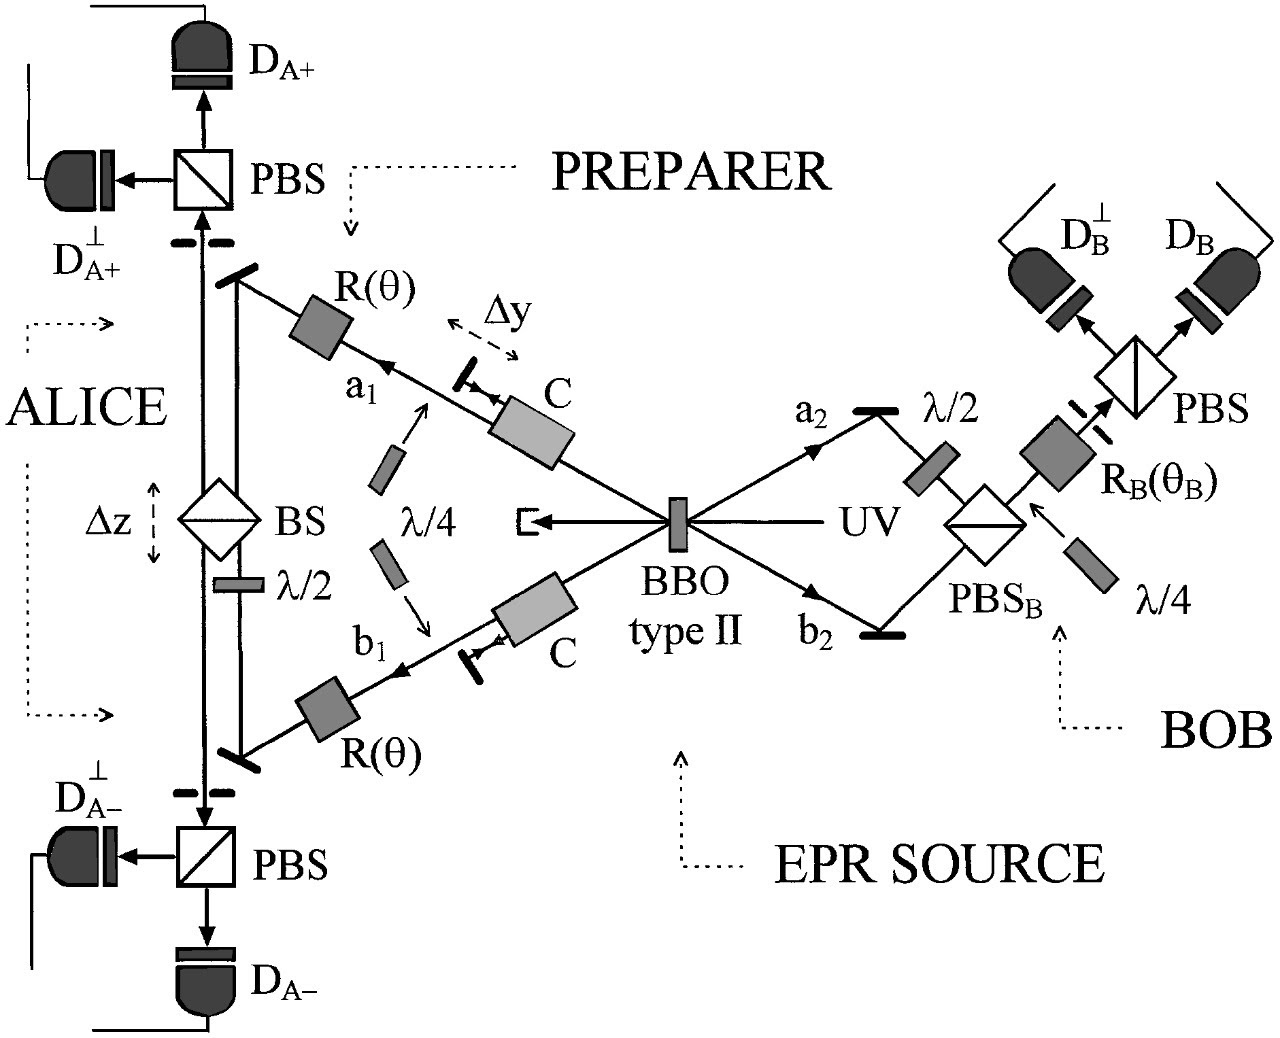
\includegraphics[width=0.5\textwidth]{figures/setup_diagram.jpg}
    \caption{Diagram of experimental setup showing the separate roles of the preparer, Alice, and Bob.}
    \label{fig:experimental_setup}
\end{figure}

\subsubsection{\textbf{The Preparer: Encoding the Unknown State}}
A strict logical distinction is maintained between the Preparer and Alice. To ensure the state $|\phi\rangle$ remains fundamentally "unknown," the Preparer encodes it onto photon 1's polarization before it reaches Alice's apparatus. This relies on local unitary operations on paths $a_1$ and $b_1$:

\begin{itemize}
    \item \textbf{Polarization Initialization:} Photon 1 enters with an initial defined polarization (typically vertical, $|v\rangle_1$).
    \item \textbf{Unitary Manipulation:} Quarter-wave plates and Fresnel rhomb rotators (R) transform this into a general pure state: $|\phi\rangle=\alpha|v\rangle_1+\beta|h\rangle_1$.
    \item \textbf{Path Independence:} Operating identically on paths $a_1$ and $b_1$, the polarization state effectively factors out of the path entanglement. 
\end{itemize}

This yields a global tripartite system where the unknown polarization is carried by the path-entangled photon 1:
$$|\Psi_{total}\rangle=\frac{1}{\sqrt{2}}(|a_1\rangle|a_2\rangle+|b_1\rangle|b_2\rangle)(\alpha|v\rangle_1+\beta|h\rangle_1)|h\rangle_2$$

\subsubsection{\textbf{Alice's BSM Engine: Interferometric Bell State Measurement}}
Alice’s Bell State Measurement (BSM) interferometer projects photon 1's bipartite state onto four orthogonal path-polarization Bell states:
$$|c^\pm\rangle=\frac{1}{\sqrt{2}}(|a_1\rangle|v\rangle_1\pm|b_1\rangle|h\rangle_1)$$
$$|d^\pm\rangle=\frac{1}{\sqrt{2}}(|a_1\rangle|h\rangle_1\pm|b_1\rangle|v\rangle_1)$$

Prior to entering a 50:50 beam splitter (BS), a Fresnel rhomb in path $b_1$ induces a $90^\circ$ polarization rotation. This ensures path and polarization degrees of freedom are properly aligned for interference. The BS then acts as a unitary operator, mapping distinct path-polarization correlations to specific output ports. 

The BS is mounted on a micrometrical stage to precisely tune the path-length difference ($\Delta z$). Alignment is confirmed by "interference dips" in coincidence count rates, signifying spatiotemporal wave packet overlap.

\textbf{Mechanics of Detection:} Polarizing beam splitters (PBS) sort the emerging photons into four avalanche photodiode detectors ($D_{A+}, D_{A+}^\perp, D_{A-}, D_{A-}^\perp$). Detector coincidences unambiguously project onto the Bell basis:
\begin{itemize}
    \item A detection at $D_{A+}^\perp$ or $D_{A-}^\perp$ identifies states $|c^\pm\rangle$.
    \item A detection at $D_{A+}$ or $D_{A-}$ identifies states $|d^\pm\rangle$.
\end{itemize}
This projective measurement dictates the unitary operation Bob must perform to reconstruct the initial state.

\subsubsection{Bob’s Station: Reconstructing the Teleported State}
At the receiving station, photon 2 arrives via trajectories $a_2$ and $b_2$. To resolve the path entanglement, polarization in path $a_2$ is orthogonally rotated by $90^\circ$ via a half-wave plate before recombining with path $b_2$ at the polarizing beam splitter ($PBS_B$).

Bob employs \textit{passive reconstruction}. Rather than dynamically rotating the state using active electro-optic switches, he reorients his measurement basis to verify the teleported state based on Alice's classical transmission.

\textbf{Unitary Transformation Logic:}
\begin{itemize}
    \item \textbf{Linear States:} Bob adjusts his Fresnel rhomb ($R_B$) to an angle $\theta_B$, determined by Alice’s Bell state outcome.
    \item \textbf{Elliptical States:} Bob inserts a quarter-wave plate at angle $\gamma_B$ to map the expected elliptical state back into an observable linear basis.
    \item \textbf{Phase Matching:} Bob uses a micrometrical stage to tune $\Delta y$, ensuring paths satisfy the phase-matching criteria for high-fidelity verification.
\end{itemize}

\subsection{The Verdict: Beating the Classical Limit}
To rigorously validate quantum teleportation, the experimental fidelity ($S$)—representing the average probability of the teleported state passing verification—must strictly exceed the classical communication limit of $0.75$. Surpassing this threshold empirically proves that entanglement was utilized as a non-local resource.In the 1998 experiment, $S$ was derived through a comprehensive sampling process across three equally spaced linear polarization settings ($0^\circ, 120^\circ, \text{ and } -120^\circ$). To ensure a representative result on the Bloch sphere, each of these three states was assigned a weight of $1/3$, while each of the four possible Bell state measurement outcomes was weighted equally at $1/4$. The final observed fidelity of $0.853 \pm 0.012$ exceeds the classical bound by eight standard deviations. This result robustly confirms that the dual-degree-of-freedom architecture functioned as a unified quantum processor, providing definitive empirical proof of the successful teleportation of unknown pure quantum states. 
\label{sec:Experimental Implementation}



\section{Variants of Quantum Teleportation}

\subsection{Optical Modes System: Continuous-Variable Teleportation}

In the previous chapter, we explored the standard quantum teleportation protocol, which is based on discrete-variable (DV) systems and uses photonic qubits as the information carriers. Now, it is reasonable to ask the following question: can we construct a teleportation protocol in an infinite-dimensional Hilbert space instead of only a two-dimensional one?

The answer is yes. Instead of encoding quantum information in a two-level system such as
Eq.\ref{Eq: qubit}. Continuous-variable (CV) teleportation uses quantum states of optical modes. A single optical mode is mathematically equivalent to a quantum harmonic oscillator, whose Hilbert space is spanned by the infinite set of Fock states: $\ket{0}, \ket{1}, \ket{2}, \cdots $. Therefore, the state to be teleported is no longer restricted to a qubit. It can be an arbitrary state of one mode of the electromagnetic field, described by continuous quadrature variables. 
Now I'll give example for CV telelporation using optical modes.

For an optical mode with annihilation  operator $\hat{a}$, we define the field quadratures
\begin{equation}
    \hat{x} = \frac{1}{\sqrt{2}}(\hat{a}+\hat{a}^{\dagger}),
    \qquad
    \hat{p} = \frac{1}{i\sqrt{2}}(\hat{a}-\hat{a}^{\dagger});
    \quad 
    [\hat{x},\hat{p}] = i
\end{equation}
which are analogous to the position and momentum operators of a harmonic oscillator. 
A quantum state of the optical mode can then be represented in phase space by a Wigner function
\begin{equation}
    W_{\text{in}}(\alpha
    ) ~;~ \alpha = x+ip.
    \label{Eq:Wigner_function_input}
\end{equation}


Thus, we get the continuous-variable version of the EPR state, which is charaterzied by $x$ and $p$ field quadratures. 
And in reality we cannot create a perfect correlated EPR state between Alices and Bobs because that would require infinite squeezing and therefore infinite energy.
Instead, we often adopt convential correlation relations
used by Braunstein and Kimble\cite{PhysRevLett.80.869}. With $x_1$ and $p_1$ being the quadratures of Alice's mode, and $x_2$ and $p_2$ being the quadratures of Bob's mode, the EPR correlations can be expressed as
\begin{equation}
    x_1 + x_2 \rightarrow 0,
    \qquad
    p_1 - p_2 \rightarrow 0.
    \label{Eq:Correlation}
\end{equation}

With the physics defined clearly we can now see how the continuous-variable teleportation protocol works. 
Initially, Alice is given an unknown input state as Eq.\ref{Eq:Wigner_function_input},
which she wants to teleport to Bob. And Alice and Bob share an EPR state with the correlation in Eq.\ref{Eq:Correlation}. 

Starting the teleportation, Alice first combines the unknown input mode with her half of the EPR pair on a 50/50 beam splitter(the lower beam splitter in the green area in Fig.\ref{fig:CV_teleportation_diagram}).

\begin{figure}[h]
    \centering
    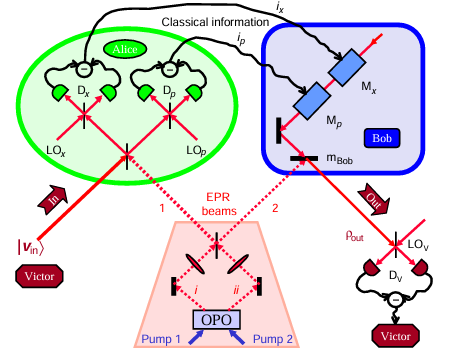
\includegraphics[width=0.5\textwidth]{figures/Unconditional teleportation_setup.png}3
    \caption{Diagram of the continuous-variable teleportation experiment by Braunstein and Kimble \cite{PhysRevLett.80.869}.}
    \label{fig:CV_teleportation_diagram}
\end{figure}

The beam splitter produces two output modes,
\begin{equation}
    \hat{a}_{a} = \frac{1}{\sqrt{2}}(\hat{a}_{1}+\hat{a}_{\text{in}}),
    \qquad
    \hat{a}_{b} = \frac{1}{\sqrt{2}}(\hat{a}_{1}-\hat{a}_{\text{in}}).
\end{equation}



She then performs balanced homodyne measurements on these two modes. Specifically, she measures the quadrature combinations
\begin{equation}
    x_a = \frac{1}{\sqrt{2}}(x_{\text{in}}-x_1),
    \qquad
    p_b = \frac{1}{\sqrt{2}}(p_{\text{in}}+p_1).
\end{equation}
These measurement outcomes are ordinary classical numbers. Alice sends the values of $x_a$ and $p_b$ to Bob through a classical communication channel($i_x$ and $i_p$ in Fig.\ref{fig:CV_teleportation_diagram}).

After receiving Alice's measurement results, Bob applies a phase-space displacement to his optical mode. 
In terms of the complex amplitude, this displacement can be written as
\begin{equation}
    \alpha_{\text{out}}
    =
    \alpha_2 + \sqrt{2}(x_a - i p_b)
    =
    g\alpha_{\text{in}} + [(x_2 -gx_1) + i(p_2 - g p_1)].
\end{equation}
where $g$ describes Bob's (suitably normalized) gainfor the transformation from photocurrent tooutput field.

Using the EPR correlations in Eq.\ref{Eq:Correlation}, 
we can see why this reconstructs the input state. For the $x$ and $p$ quadrature,
\begin{equation}
\left\{
\begin{aligned}
x_{\text{out}}
&= x_2 + \sqrt{2}x_a
 = x_2 + x_1 + x_{\text{in}}
 \approx x_{\text{in}}, \\[4pt]
p_{\text{out}}
&= p_2 - \sqrt{2}p_b
 = p_2 - p_1 + p_{\text{in}}
 \approx p_{\text{in}}.
\end{aligned}
\right.
\end{equation}
Thus, Bob's output mode becomes a copy of Alice's unknown input state, up to the error caused by finite squeezing and imperfect detection.
In terms of the Wigner function, the output state is a convolution of the input state with a Gaussian noise:
\begin{equation}
    W_{\text{out}}(\alpha)
    =
    W_{\text{in}}(\alpha) * G_s(\alpha).
\end{equation}
Here, $G_s$ is a Gaussian distribution whose variance is determined by the amount of squeezing. For ideal detection,
\begin{equation}
    s = e^{-2r},
\end{equation}
where $r$ is the squeezing parameter. Therefore, in the limit of infinite squeezing,
\begin{equation}
    r \rightarrow \infty,
    \qquad
    e^{-2r} \rightarrow 0,
\end{equation}
the Gaussian noise vanishes and the output state becomes exactly equal to the input state:
\begin{equation}
    W_{\text{out}}(\alpha) \rightarrow W_{\text{in}}(\alpha).
\end{equation}

For realistic detectors, however, the output contains additional noise due to imperfect detection efficiency. If the detector amplitude efficiency is $\eta$, the effective noise becomes

\begin{equation}
    \bar{s}
    =
    e^{-2r}
    +
    \frac{1-\eta^2}{\eta^2}.
\end{equation}

This equation shows the two main limitations of practical CV teleportation, which are finite squeezing and detector loss. 
Increasing the squeezing reduces the first term, while improving the homodyne detection efficiency reduces the second term.

Up until now, we have described the typical teleportation for continuous variables. 
Yet, we didn't seems to mention how significant this protocal is or how significant "quantum teleportation" is in general. 
A useful way to understand the importance is to compare quantum teleportation with a purely classical strategy.
If there is no entanglement between the shared state, corresponding to $r=0$, Alice can only measure the input state and tell Bob what state to prepare.
However, because $\hat{x}$ and $\hat{p}$ do not commute, Alice cannot measure both quadratures perfectly at the same time. The measurement necessarily adds quantum noise.
Bob's reconstruction also adds noise. Therefore, the classical measure-and-prepare protocol cannot perfectly reproduce the input quantum state. 
In contrast, when $r>0$, Alice and Bob share genuine EPR entanglement, and the teleportation fidelity can exceed what's possible with classical methods (see Fig.\ref{fig:fidelity_plot}).

\begin{figure}[h]
    \centering
    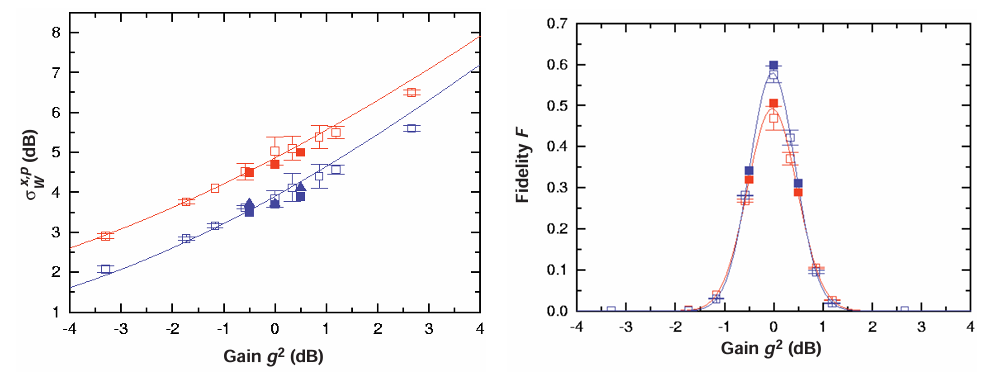
\includegraphics[width=1\textwidth]{figures/Quantum vs classical.png}
    \caption{Experimental result by Braunstein and Kimble\cite{PhysRevLett.80.869}. The left figure is the variance of the Bob's state vesus $g^2$, and the right figure shows the fidelity versus $g^2$.
     The orange line indicates the classical teleporation and blue indicates the quantum teleportation.}
    \label{fig:fidelity_plot}
\end{figure}

In a nutshell, continuous-variable teleportation extends the original teleportation idea from finite-dimensional qubits to infinite-dimensional optical modes. 
The unknown state is encoded in the quadrature amplitudes of an electromagnetic field mode, which is easily to measure and recreate experimentally. 
The quality of teleportation is limited by finite squeezing and detector inefficiency, but with sufficient squeezing the protocol can teleport genuinely nonclassical optical states with fidelity beyond any classical measure-and-prepare scheme.
\newpage

%%%%%%%%%%%%%%%%%%%%%%%%%%%%%%%%%%%%%%%%%
\subsection{Atomic Ensemble Systems}
\label{subsec:atomic_ensemble_systems}

Unlike using photons as the source of quantum information like we discussed above, we can also use atoms as the information carriers.
Atomic ensambles in nature are better suited for local storage and synchronization, while photons are better suited for long-distance transmission. 
Before  true atomic ensembles, it is useful to first mention an important precursor experiment: the generation of Einstein--Podolsky--Rosen (EPR) pairs of atoms by Hagley \textit{et al.} \cite{Hagley1997}. Although this experiment used two individual Rydberg atoms rather than a many-atom ensemble, it demonstrated a key idea for matter-based teleportation: massive particles can be entangled in a controlled way through their interaction with a quantized electromagnetic field. In the experiment, two rubidium atoms passed one after another through a high-\(Q\) microwave cavity. The first atom was initially prepared in an excited circular Rydberg state \(\ket{e}\), the second in a lower state \(\ket{g}\), and the cavity was initially in the vacuum state \(\ket{0}\). The initial state was therefore
\begin{equation}
    \ket{\Psi_{\mathrm{in}}}
    =
    \ket{e_1,g_2,0}.
\end{equation}
The first atom interacted with the cavity for a time corresponding to a \(\pi/2\) Rabi pulse. This produced a superposition in which the first atom either remained excited and left the cavity empty, or emitted one photon into the cavity:
\begin{equation}
    \ket{\Psi'}
    =
    \frac{1}{\sqrt{2}}
    \left(
        \ket{e_1,g_2,0}
        -
        \ket{g_1,g_2,1}
    \right).
\end{equation}
The second atom then interacted with the cavity for a \(\pi\) pulse. If the photon was present, the second atom absorbed it and was promoted from \(\ket{g}\) to \(\ket{e}\). After this process, the cavity returned to the vacuum state, while the two atoms were left in the entangled EPR state
\begin{equation}
    \ket{\Psi_{\mathrm{EPR}}}
    =
    \frac{1}{\sqrt{2}}
    \left(
        \ket{e_1,g_2}
        -
        \ket{g_1,e_2}
    \right).
\end{equation}
Thus, the cavity field acted as an intermediate quantum bus: it started and ended in the vacuum state, but during the process it mediated the entanglement between the two atoms. The atoms were separated by a distance on the order of a centimeter, showing that EPR-type entanglement could be produced between spatially separated massive particles \cite{Hagley1997}. This result is conceptually important for teleportation because quantum teleportation requires a shared entangled resource. Hagley's experiment showed that such an entangled resource can be engineered between material systems rather than only between photons.

The connection to atomic ensemble teleportation becomes clearer when one replaces individual atoms by collective atomic excitations. In an ensemble, the quantum information is not stored in one specific atom, but in a coherent collective mode shared among many atoms. This collective enhancement increases the effective coupling between light and matter and allows the ensemble to behave like a single effective quantum memory. Depending on the encoding, atomic ensembles can be used either in a continuous-variable framework or in a discrete-variable spin-wave framework.

In the continuous-variable approach, the collective spin of an ensemble is treated as an effective harmonic oscillator. A representative experiment was performed by Sherson \textit{et al.}, in which a quantum state of light was teleported onto a macroscopic atomic ensemble containing approximately \(10^{12}\) cesium atoms \cite{Sherson2006}. The atoms were optically pumped into a coherent spin state with a large mean spin along the \(x\)-direction. The two transverse spin components could then be normalized as canonical variables,
\begin{equation}
    \hat{X}_A =
    \frac{\hat{J}^{\mathrm{rot}}_y}{\sqrt{J_x}},
    \qquad
    \hat{P}_A =
    \frac{\hat{J}^{\mathrm{rot}}_z}{\sqrt{J_x}},
\end{equation}
where \(J_x\) is the large mean collective spin. Under the condition that the transverse spin fluctuations are small compared with \(J_x\), these variables approximately satisfy
\begin{equation}
    [\hat{X}_A,\hat{P}_A]=i.
\end{equation}
This makes the atomic ensemble mathematically analogous to an optical mode with quadrature operators.

The entanglement resource in the Sherson experiment was created by sending a strong off-resonant light pulse through the atomic ensemble. Through a Faraday-type interaction, the polarization quadratures of the outgoing light became entangled with the collective spin quadratures of the atoms. Physically, the atomic spin rotated the polarization of the light, while the light also acted back on the atoms through the ac Stark effect. After this interaction, the outgoing light pulse was sent to Alice and mixed on a \(50/50\) beamsplitter with the unknown optical state to be teleported. Alice then performed a Bell measurement using polarization homodyne detection. The resulting classical photocurrents were sent to Bob, who applied radio-frequency magnetic-field pulses to the atomic ensemble. These pulses displaced the collective spin variables according to Alice's measurement result.

Ideally, the feed-forward operation maps the input optical quadratures onto the atomic ensemble,
\begin{equation}
    \hat{Y},\hat{Q}
    \longrightarrow
    \hat{X}^{\mathrm{tele}}_A,\hat{P}^{\mathrm{tele}}_A ,
\end{equation}
where \(\hat{Y}\) and \(\hat{Q}\) are the quadratures of the input light field, and \(\hat{X}^{\mathrm{tele}}_A\), \(\hat{P}^{\mathrm{tele}}_A\) are the final teleported atomic variables. The original optical state is not transferred by a direct classical copying process. Instead, the pre-existing light--matter entanglement, the Bell measurement, the classical communication, and the conditional spin displacement together reproduce the input quantum state in the atomic ensemble.

The performance of the teleportation is quantified by the fidelity between the input optical state and the reconstructed atomic state. Sherson \textit{et al.} reported deterministic teleportation of coherent states with fidelities
\begin{equation}
    F = 0.60 \pm 0.02
    \qquad
    \text{for}
    \qquad
    \bar{n}=5,
\end{equation}
and
\begin{equation}
    F = 0.58 \pm 0.02
    \qquad
    \text{for}
    \qquad
    \bar{n}=20.
\end{equation}
These values exceeded the corresponding classical benchmarks, showing that the process could not be explained as a purely classical measure-and-prepare transfer \cite{Sherson2006}. The final atomic state was verified by sending a second strong pulse through the ensemble and reconstructing the atomic quadratures from the outgoing light.

A later development extended this idea from light-to-matter teleportation to matter-to-matter teleportation. Krauter \textit{et al.} demonstrated deterministic continuous-variable teleportation between two distant macroscopic atomic ensembles at room temperature \cite{Krauter2013}. In this case, light was used to distribute entanglement between two material systems, and a collective spin state encoded in one ensemble was teleported onto another ensemble. This result is conceptually close to the original goal of a quantum network: information begins in a stationary matter system, is transferred through a light-mediated entangled channel, and ends in another stationary matter system.

Atomic ensembles can also be used in a discrete-variable framework. Here the relevant excitation is a single collective spin wave. Suppose all atoms are initially in the ground state \(\ket{g}\). A weak write pulse can create a Stokes photon together with one collective excitation in another long-lived atomic state \(\ket{s}\). The spin-wave state can be written as
\begin{equation}
    \ket{1}_{\mathrm{sw}}
    =
    \frac{1}{\sqrt{N}}
    \sum_{j=1}^{N}
    e^{i\mathbf{k}_{\mathrm{sw}}\cdot \mathbf{r}_j}
    \ket{g_1 g_2 \cdots s_j \cdots g_N},
\end{equation}
where \(N\) is the number of atoms, \(\mathbf{r}_j\) is the position of the \(j\)-th atom, and
\begin{equation}
    \mathbf{k}_{\mathrm{sw}}
    =
    \mathbf{k}_{\mathrm{write}}
    -
    \mathbf{k}_{\mathrm{Stokes}}
\end{equation}
is the spin-wave wave vector. The phase factor determines the spatial mode of the collective excitation. During readout, a read pulse converts the spin wave back into an anti-Stokes photon with the phase-matching condition
\begin{equation}
    \mathbf{k}_{\mathrm{anti-Stokes}}
    =
    \mathbf{k}_{\mathrm{read}}
    +
    \mathbf{k}_{\mathrm{sw}} .
\end{equation}
Therefore, the geometry of the write and read beams determines both the stored memory mode and the direction of the retrieved photon. Atomic motion can destroy the phase coherence of the spin wave, so cold atoms, long-wavelength spin waves, and carefully chosen beam geometries are important for extending the memory lifetime.

This discrete-variable picture is closely related to the DLCZ quantum repeater protocol proposed by Duan, Lukin, Cirac, and Zoller \cite{Duan2001}. In that protocol, entanglement between remote atomic ensembles is generated probabilistically. A weak write pulse creates a photon--spin-wave pair with small probability. Detection of the emitted photon heralds the presence of a collective spin excitation. By interfering photons from two remote ensembles on a beamsplitter, one can herald entanglement between the distant memories. Once such an entangled memory pair is available, teleportation can be performed by a Bell-state measurement involving the input qubit and one part of the entangled resource.

This idea was realized in memory-built-in teleportation experiments. Chen \textit{et al.} demonstrated teleportation of an unknown photonic polarization qubit onto a remote atomic ensemble, where the teleported state was stored as a collective atomic excitation and later read out \cite{Chen2008}. Bao \textit{et al.} later demonstrated quantum teleportation between two remote atomic-ensemble quantum memories connected by optical fiber \cite{Bao2012}. In that experiment, each node contained approximately \(10^8\) rubidium atoms. The spin-wave state of one ensemble was converted into a propagating photon and subjected to a Bell-state measurement with another photon entangled with the second ensemble. Successful two-photon detection heralded the teleportation event, with an average fidelity reported as \(88(7)\%\).

The continuous-variable and discrete-variable approaches have complementary advantages. Continuous-variable teleportation can be deterministic and naturally uses homodyne detection, making it well suited for Gaussian optical states and collective spin variables. However, high fidelity requires strong light--matter coupling, low optical loss, accurate feed-forward, and long atomic coherence time. Discrete-variable teleportation is naturally compatible with single-photon qubits and heralded quantum repeaters, but it is probabilistic because success depends on photon detection events. In both approaches, the main experimental limitations are optical loss, detector inefficiency, atomic decoherence, imperfect mode matching, and imperfect state preparation.

Overall, atomic ensemble systems show how quantum teleportation can become a practical interface between communication and storage. The earlier Rydberg-atom EPR experiment demonstrated that entanglement between massive particles can be engineered through controlled atom--field interaction. Later ensemble experiments extended this idea to macroscopic matter systems, where collective spin states can store, receive, and transmit quantum information. Atomic ensembles are therefore not merely passive memories; they are active quantum network nodes capable of entanglement generation, teleportation, storage, and retrieval.


\subsection{Solid-State System}

The optical-mode and atomic-ensemble systems discussed above demonstrate that quantum teleportation can be implemented in very different physical platforms. A third important direction is the solid-state system, where the quantum information is stored and processed in artificial quantum devices fabricated on a chip. In particular, superconducting circuits provide a promising solid-state platform because qubits, resonators, gates, measurements, and real-time control electronics can be integrated into a single circuit architecture. Instead of using freely propagating photons or naturally occurring atoms, this approach uses engineered macroscopic quantum systems whose quantum states behave like controllable two-level systems.

A representative experiment was demonstrated by Steffen \textit{et al.}, who realized deterministic quantum teleportation with feed-forward in a superconducting circuit. The system consists of three superconducting transmon qubits, denoted as $Q_1$, $Q_2$, and $Q_3$, coupled to three superconducting coplanar waveguide resonators. In the teleportation protocol, $Q_1$ is the qubit carrying the unknown input state
\begin{equation}
    |\psi_{\mathrm{in}}\rangle = \alpha |0\rangle + \beta |1\rangle ,
\end{equation}
while $Q_2$ and $Q_3$ are first prepared as an entangled Bell pair. Here $Q_1$ and $Q_2$ belong to the sender side, and $Q_3$ acts as the receiver qubit. Although the qubits are located on the same superconducting chip, the state is not transferred by directly moving the physical carrier from $Q_1$ to $Q_3$. Instead, as in the standard teleportation protocol, the transfer relies on a shared entangled resource and classical information obtained from a Bell-state measurement.

The protocol begins by preparing an entangled state between $Q_2$ and $Q_3$, for example
\begin{equation}
    |\Phi^+\rangle_{23}
    =
    \frac{1}{\sqrt{2}}
    \left(
    |00\rangle_{23}
    +
    |11\rangle_{23}
    \right).
\end{equation}
This entangled pair plays the same role as the EPR pair in the original teleportation proposal. After this shared resource is created, the unknown state $|\psi_{\mathrm{in}}\rangle$ is prepared on $Q_1$. The sender then performs a Bell-state measurement on $Q_1$ and $Q_2$. In the ideal circuit model, this Bell measurement can be understood as a transformation from the Bell basis to the computational basis, followed by ordinary qubit readout. Experimentally, Steffen \textit{et al.} implemented the required two-qubit operations using controlled-PHASE gates and single-qubit microwave rotations. The controlled-PHASE gates are generated by tuning the transition frequencies of the transmon qubits with fast flux pulses, while the single-qubit rotations are driven by microwave pulses.

After the Bell-state measurement, the receiver qubit $Q_3$ is projected into a state related to the original input state by a Pauli operation:
\begin{equation}
    |\psi_{\mathrm{out}}\rangle
    =
    \{ I, X, Z, \tilde{Y} \}
    |\psi_{\mathrm{in}}\rangle ,
\end{equation}
where the required correction depends on the two classical bits obtained from the Bell measurement. Therefore, the output state is not always immediately equal to $|\psi_{\mathrm{in}}\rangle$; it is equal up to a known single-qubit rotation. To complete the teleportation deterministically, the experiment must identify which Bell-state outcome occurred and then apply the corresponding correction to $Q_3$. This final conditional correction is called feed-forward. It is conceptually different from feedback: feedback acts back on the same system that was measured, while feed-forward uses the measurement result from one part of the system to control another part.

A key achievement of this solid-state implementation is that it does not merely post-select one successful outcome. In many optical teleportation experiments, only part of the Bell basis can be distinguished, so the protocol succeeds only probabilistically. In this superconducting circuit experiment, Josephson parametric amplifiers were used to perform high-fidelity single-shot measurements. The measurement outcome from the sender qubits was processed in real time by field-programmable gate array (FPGA) electronics, which then triggered the appropriate microwave pulse on $Q_3$. In this way, the experiment implemented deterministic teleportation with active feed-forward, using all four possible Bell-measurement outcomes.

The reported results show that the teleported state fidelities are above the classical limit. For post-selected teleportation, the average output-state fidelity was about $81.7\%$, with an average process fidelity of about $72.0\%$. When all four Bell-state outcomes were distinguished deterministically, the average output-state fidelity was about $77.1\%$, with a process fidelity of about $65.5\%$. When real-time feed-forward was included, the directly measured deterministic state-transfer fidelity was about $68.8\%$, still above the classical threshold of $2/3$ for state teleportation. The lower fidelity in the full feed-forward case mainly came from imperfect qubit coherence, gate errors, readout errors, and the finite delay required for real-time measurement processing and conditional control.

The importance of this experiment is that it shows quantum teleportation can be implemented inside a scalable chip-based architecture. Compared with optical systems, superconducting circuits are not naturally suited for long-distance transmission, since microwave photons are harder to send over free space or ordinary optical fibers. However, they have strong advantages for quantum computation: qubits can be fabricated lithographically, coupled through resonators, controlled with fast microwave pulses, and measured with integrated cryogenic electronics. The experiment teleported states between two superconducting qubits separated by several millimeters on a chip and operated at a rate of approximately $10^4 \ \mathrm{s}^{-1}$, much faster than many earlier teleportation demonstrations.

More broadly, solid-state teleportation is significant because it connects teleportation directly to the architecture of quantum processors. In a quantum computer, teleportation is not only a communication protocol; it can also be used as a tool for quantum gates, state transfer, modular quantum computing, and quantum error correction. The demonstrated feed-forward is especially important because error correction also requires measurement outcomes to be processed in real time and converted into conditional quantum operations. Therefore, the superconducting solid-state system provides a bridge between the conceptual teleportation protocol and practical quantum information processing on a chip.

In summary, the solid-state implementation of quantum teleportation replaces photons or atoms with superconducting artificial atoms embedded in a microwave circuit. The essential ingredients remain the same: an unknown input state, a shared entangled pair, a Bell-state measurement, classical information, and a conditional correction. The main achievement of the superconducting platform is that all these steps, including deterministic Bell-state readout and feed-forward, can be realized in an integrated circuit. This makes solid-state teleportation an important step toward scalable quantum processors and future quantum communication between superconducting modules.

\section{Advances in Quantum Teleportation}

\label{sec:Advances in Quantum Teleportation}
%%%%%%%%%%%%%%%%%%%%%%%%%%%%%%%%%%%%%%%%%%%%%%%%%%%

\subsection{Quantum Teleportation for Quantum Communication}

One of the most important advances of quantum teleportation is its application to
long-distance quantum communication. In ordinary communication, information is
carried by a physical signal, such as an electromagnetic wave or an optical pulse.
However, when the information is an unknown quantum state, it cannot simply be
measured and copied because of the no-cloning theorem. Quantum teleportation
provides a way to transfer this unknown state from one system to another by using
two resources: a shared entangled state and a classical communication channel.

A clear experimental example is the ground-to-satellite quantum teleportation
experiment performed using the Micius satellite \cite{ren2017ground}. In this
experiment, the quantum state to be teleported was encoded in the polarization of
a single photon,
\begin{equation}
    \ket{\chi}_1 = \alpha \ket{H}_1 + \beta \ket{V}_1,
    \qquad |\alpha|^2 + |\beta|^2 = 1,
\end{equation}
where \(\ket{H}\) and \(\ket{V}\) represent horizontal and vertical polarization.
These two polarization states play the role of the qubit basis states
\(\ket{0}\) and \(\ket{1}\). The ground station also prepared an entangled photon
pair in the Bell state
\begin{equation}
    \ket{\phi^+}_{23}
    =
    \frac{1}{\sqrt{2}}
    \left(
        \ket{H}_2\ket{H}_3
        +
        \ket{V}_2\ket{V}_3
    \right).
\end{equation}
Photon 2 remained at the ground station, while photon 3 was sent through a
free-space optical uplink to the satellite. The ground station then performed a
Bell-state measurement on photons 1 and 2. Depending on the Bell-state
measurement result, the state of photon 3 became either the desired state
\(\ket{\chi}\), or a state related to it by a known unitary correction such as a
\(\pi\)-phase shift. Therefore, the unknown quantum state was not physically
carried by photon 1 to the satellite; instead, it was reconstructed in the distant
photon 3 by using entanglement plus classical information.

This experiment is important because it addresses the main difficulty of
long-distance quantum communication: photon loss. Previous teleportation
experiments using optical fibers or terrestrial free-space channels were limited
to roughly the hundred-kilometer scale because loss increases strongly with
distance. A satellite link reduces this problem because most of the propagation
path is through empty space rather than through an absorbing medium. In the
Micius experiment, the teleportation distance varied from about \(500\) km to
\(1400\) km, with a measured channel loss ranging from about \(41\) dB to
\(52\) dB. Even with this large loss, the experiment successfully teleported six
input states chosen from mutually unbiased bases on the Bloch sphere:
\[
    \ket{H},\quad \ket{V},\quad \ket{+},\quad \ket{-},\quad \ket{R},\quad \ket{L}.
\]
The measured average teleportation fidelity was
\[
    F = 0.80 \pm 0.01,
\]
which is clearly above the classical limit of \(2/3\). This means that the result
cannot be explained by a classical strategy based only on measuring the input
state and sending classical information.

From an experimental point of view, the propagation direction, or wave vector
\(\mathbf{k}\), is also crucial. The qubit itself is encoded in polarization, which is
defined transverse to the photon's propagation direction. However, in a
ground-to-satellite link, the direction of propagation is constantly changing
because the satellite moves rapidly relative to the ground station. Atmospheric
turbulence also causes beam wandering and beam broadening. Therefore, the
experiment required a narrow-divergence transmitting telescope and a precise
acquiring, pointing, and tracking system. In addition, polarization compensation
using wave plates was needed so that the polarization qubit remained well-defined
during transmission.

This result shows that quantum teleportation is not only a conceptual consequence
of entanglement, but also a practical building block for a future quantum internet.
In such a network, teleportation could be combined with entanglement distribution,
quantum memories, and entanglement swapping to connect distant quantum nodes.
The ground-to-satellite experiment is therefore an important step from laboratory
teleportation toward global-scale quantum communication.

\subsection{Quantum Gate Teleportation for Quantum Computing}

While standard quantum teleportation transfers an unknown quantum state from one system to another, quantum gate teleportation (QGT) extends the same principle to quantum operations. Instead of physically moving a qubit from one processor to another, QGT uses a previously shared entangled state, local operations, measurement, and classical feed-forward to implement a non-local gate between distant qubits. This idea is especially important for quantum computing, because large-scale quantum processors require many qubits with high connectivity. Building a single device in which every qubit can directly interact with every other qubit is technically difficult. QGT provides an alternative route: separated quantum modules can behave as one larger processor if entangling gates can be teleported between them.

A recent experimental demonstration by Main \textit{et al.} shows how this idea can be used for distributed quantum computing across an optical network link \cite{Main2025Distributed}. In their architecture, two trapped-ion modules, labeled Alice and Bob, are separated by about two meters. Each module contains two functional types of qubits: a \textit{network qubit}, used to create remote entanglement through photons, and a \textit{circuit qubit}, used to store and process the computational quantum information. This separation of roles is essential. The network qubits interact with the optical link and generate entanglement, while the circuit qubits preserve the quantum information during the probabilistic entanglement-generation process.

The central resource is a remotely shared Bell state between the two network qubits,
\[
\ket{\Psi^+}_{N}
=
\frac{1}{\sqrt{2}}
\left(
\ket{10}+\ket{01}
\right),
\]
which is generated by photon-mediated entanglement and heralded by detector clicks. Once this entanglement has been successfully produced, local controlled-Z operations are performed inside each module between the network qubit and the local circuit qubit. The network qubits are then measured in chosen bases, and the two modules exchange the measurement outcomes through a classical communication channel. Finally, conditional single-qubit corrections are applied to the circuit qubits. The net effect is that the circuit qubits, which are physically located in different modules, undergo a non-local controlled-Z gate,
\[
\ket{\psi_{\mathrm{in}}}_{AB}
\longrightarrow
U_{\mathrm{CZ}}\ket{\psi_{\mathrm{in}}}_{AB}.
\]
Thus, the gate is not produced by a direct physical interaction between the two circuit qubits, but by consuming the previously shared entanglement.

The important point is that the gate teleportation protocol is deterministic after entanglement has been heralded. Photon loss only affects whether the Bell pair is successfully created; it does not destroy the unknown computational state stored in the circuit qubits. This is a major advantage over direct photon-mediated transfer of quantum information, where loss of the photon can correspond to loss of the quantum state itself. In QGT, the quantum channel is only responsible for preparing entanglement, so failed attempts can simply be repeated until success. This makes the method more suitable for scalable architectures.

Experimentally, Main \textit{et al.} teleported a controlled-Z gate between two trapped-ion circuit qubits in separate modules and obtained an average gate fidelity of \(86.2(9)\%\). Since a controlled-Z gate combined with arbitrary single-qubit rotations forms a universal set for quantum computation, this demonstrates a basic building block for distributed quantum computing. The authors further showed that repeated rounds of QGT can be combined to form larger two-qubit operations. For example, they implemented distributed iSWAP and SWAP gates, which require two and three teleported controlled-Z gates, respectively. The measured process fidelities were \(70(2)\%\) for iSWAP and \(64(2)\%\) for SWAP.

Beyond individual gates, the experiment also demonstrated a small distributed quantum algorithm. The authors implemented a two-qubit version of Grover's search algorithm, where one teleported gate acts as the oracle and another teleported gate acts as the diffusion operation. For the four possible marked states,
\[
a \in \{00,01,10,11\},
\]
the distributed processor found the correct state with an average success probability of \(71(1)\%\). Although this is still far from fault-tolerant quantum computation, it is significant because it demonstrates that quantum teleportation can be used not only to transfer states, but also to execute multi-gate algorithms across separated quantum processors.

This result changes the role of teleportation in quantum computing. In early discussions, teleportation was often introduced as a surprising communication protocol: an unknown state can be transferred using entanglement and classical information. In distributed quantum computing, however, teleportation becomes an engineering tool for connectivity. It allows separate quantum modules to share entangling gates without requiring all qubits to be located in the same trap, chip, or cavity. In this sense, quantum gate teleportation provides a path toward modular quantum computers, where many smaller high-quality processors are connected by optical links and operate together as one larger machine.

\section{Conclusion}

%%%%%%%%%%%%%%%%%%%%%%%%%%%%%%%%%%%%%%%%%%%%%%%%%%

\bibliographystyle{apsrev}
\bibliography{reference}

\end{document}



